\chapter{Project Delivery, Operations and BI}
\section*{Introduction}
\addcontentsline{toc}{section}{Introduction}
This chapter covers the operational delivery layer of \projectname{}. It connects follow-up, milestones, work allocation, documents, dashboards, and report generation, then closes with the Human Resources and employee area as an integration point for employee statistics, internal events, and staffing context.
\section{Sprint and Module Objective}
The objective of this module was to deliver an operational cockpit for partnership execution, with a coherent flow from project creation to monitoring, milestone planning, task tracking, and management-ready analytics.
\begin{itemize}
  \item \textbf{Project portfolio control}: list partner projects with status, health, progress, and budget indicators.
  \item \textbf{Project execution detail}: expose milestones, mini tasks, team allocations, and project documents.
  \item \textbf{Decision-support analytics}: consolidate operational data into a BI dashboard backed by a separate data warehouse.
  \item \textbf{People and HR readiness}: expose employee statistics and events, then define the integration path with the future Capgemini HR/recruitment sister project.
\end{itemize}
\section{Module Backlog}
The backlog groups the delivery module into operational capabilities rather than isolated screens. Each item links a user need to the evidence required during demonstration: portfolio visibility, project detail, milestones, tasks, allocations, documents, health analysis, BI, reports, and HR-readiness signals.
\begin{longtable}{p{1.1cm}p{4.2cm}p{6.1cm}p{2.2cm}}
  \caption{Backlog for the project delivery, BI and HR-readiness module}\label{tab:chapter5-backlog} \\
  \toprule
  ID & User story & Acceptance criteria & Priority \\
  \midrule
  \endfirsthead
  \toprule
  ID & User story & Acceptance criteria & Priority \\
  \midrule
  \endhead
  B5.1 & As an employee, I can view a portfolio of active and archived projects. & The list shows partner, project type, health, progress, budget usage, schedule status and quick access to the detail page. & High \\
  B5.2 & As a manager, I can open a project detail page. & The page presents summary metrics, timeline, health explanation, linked partner context and execution sections. & High \\
  B5.3 & As an operational user, I can track milestones. & Milestones have labels, dates, status and a visible relation to project progress. & High \\
  B5.4 & As an operational user, I can manage small execution tasks. & A lightweight task list supports ownership, completion status and blocked items without becoming a full external project-management tool. & Medium \\
  B5.5 & As a manager, I can see team allocations. & Assigned employees, roles, allocation rates and availability context are visible in the project page. & High \\
  B5.6 & As an employee, I can attach or consult project documents. & Documents are linked to the project and remain accessible from the execution workspace. & Medium \\
  B5.7 & As an analyst, I can identify weak project health signals. & The system combines delay, budget, progress, milestone and staffing signals into readable health analysis. & High \\
  B5.8 & As an analyst, I can consult BI charts from warehouse data. & BI indicators are generated from a dedicated warehouse database and aggregated on the server before rendering. & High \\
  B5.9 & As a manager, I can export reports to PDF. & Generated report content can be opened in the report workspace and exported as a PDF deliverable. & Medium \\
  B5.10 & As an HR user, I can consult employee and event signals. & The HR area exposes employee counts, roles, events and readiness for future integration. & Medium \\
  B5.11 & As a university-partnership owner, I can treat student recruitment and CDI conversion data as partner signals. & Academic partnership performance can include internships, student recruitment operations and CDI conversions without mixing them with generic HR administration. & Medium \\
  \bottomrule
\end{longtable}
\section{Project Portfolio}
\begin{figure}[htbp]
  \centering
  \dgram{usecase-delivery}
  \caption{Use cases of the delivery, business-intelligence, and human-resources module.}
\end{figure}
\begin{itemize}
  \item \textbf{Health and progress}: on track, under observation, or at risk, with completion percentage derived from project progress and milestones.
  \item \textbf{Budget, schedule, and access}: consumption versus plan, start date, target date, delay, overdue indicators, partner organization, category, and quick navigation to the detail page.
\end{itemize}

\section{Project Detail Page}
\begin{figure}[htbp]
  \centering
  \shot{project-detail}
  \caption{Project detail workspace.}
\end{figure}
The project detail page turns the portfolio row into an execution workspace. It keeps the project summary, operational timeline, delivery health, milestones, tasks, allocation notes, and documents in one place so a manager can understand both the business context and the current execution risk without switching tools.

\subsection{Health, Progress, Budget and Schedule}
The first block gives the fast operational read: qualitative health, completion percentage, budget use, planned dates, target dates, and delay indicators. These values are designed to answer the manager's first question before the detailed lists are inspected: is the project healthy enough to continue normally, or does it require review?

\subsection{Milestones}
\begin{itemize}
  \item milestone title, description, planned date, and deadline;
  \item status such as planned, in progress, completed, or blocked, plus contribution to the overall progress view and health signals when key work is late.
\end{itemize}
\subsection{Mini Task System}
\begin{itemize}
  \item a short title, owner, and completion state;
  \item a due date when relevant, plus a blocked flag or local note for follow-up.
\end{itemize}
\subsection{Team Allocations}
\begin{itemize}
  \item staffing sufficiency, delay cause, and overload risk.
\end{itemize}
\subsection{Project Documents}
Project documents provide the evidence layer for delivery. Each document remains attached to the project context rather than scattered across shared drives, making it easier to review contracts, validation notes, meeting outputs, deliverables, or partner-provided files during a status decision. The document area is intentionally lightweight: it supports traceability and consultation without replacing a full document-management system.

\section{Project Health Analysis Signals}
Project health is not stored as an arbitrary label. The page combines delivery signals that are visible to the team: schedule delay, progress gaps, budget drift, blocked milestones, allocation pressure, missing documents, partner dependency, and repeated status drift. Figure~\ref{fig:project-health} shows the aggregation path from raw delivery signals to the final green, orange, or red health state.
\begin{figure}[H]
  \centering
  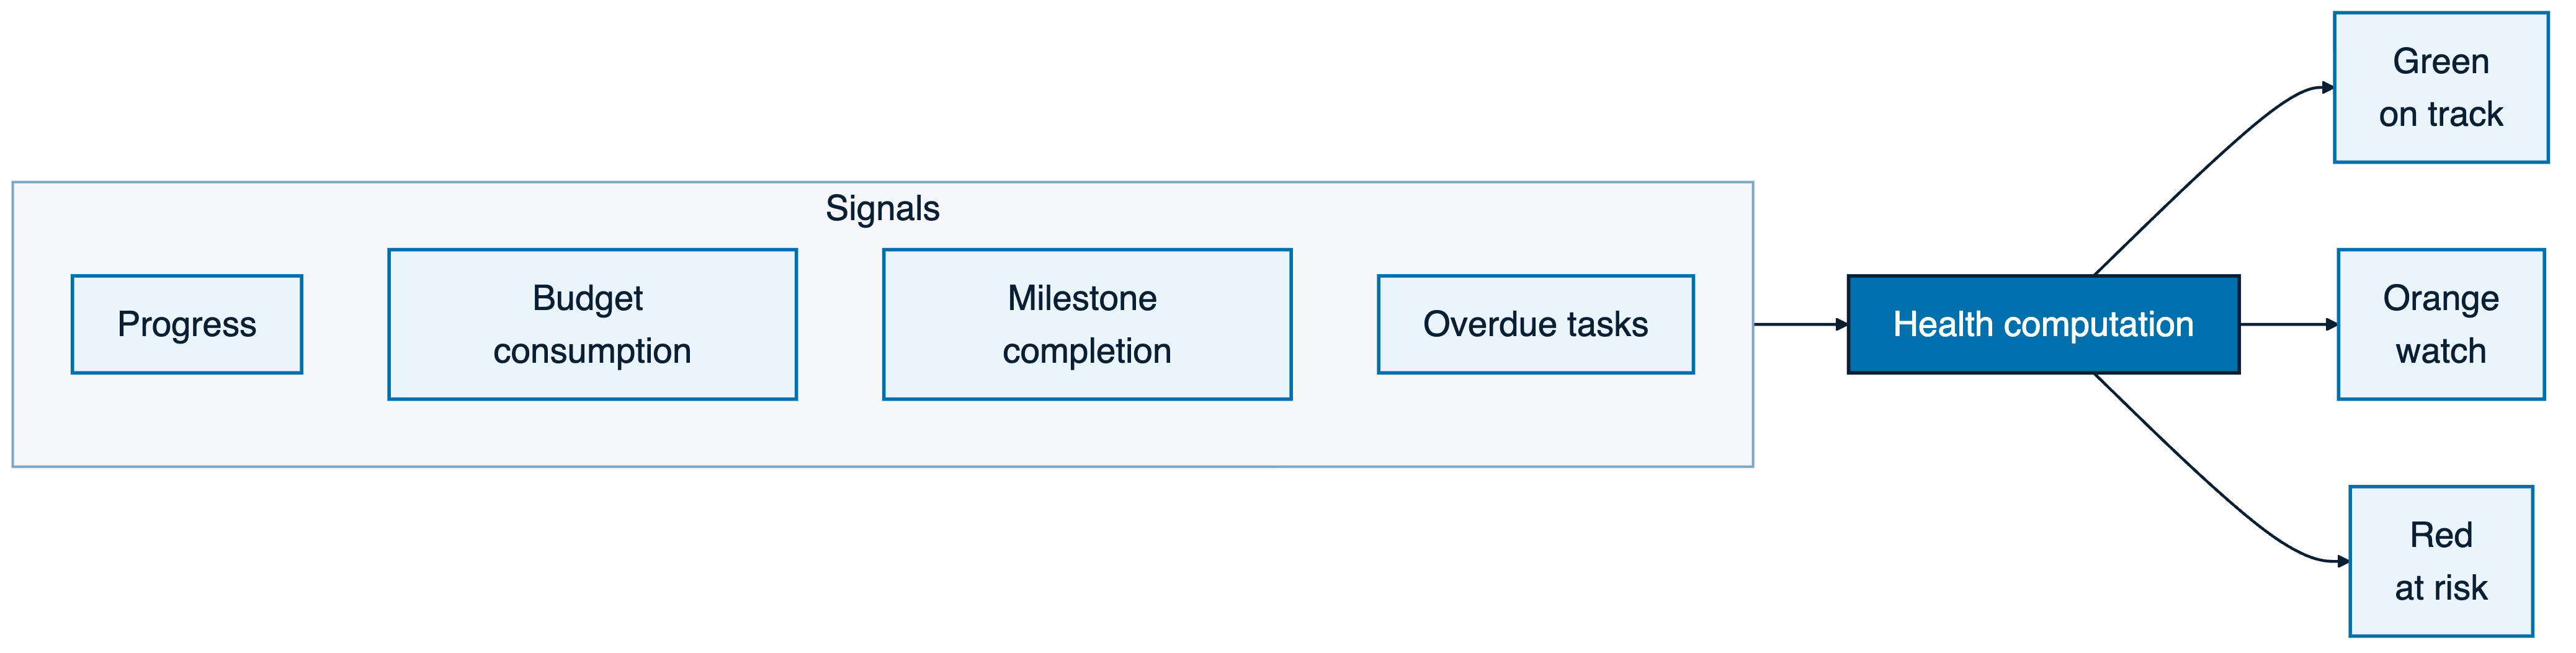
\includegraphics[width=0.84\linewidth,height=0.19\textheight,keepaspectratio]{figures/diagrams/project-health}
  \caption{Project health computed from delivery signals.}
  \label{fig:project-health}
\end{figure}
\begin{table}[H]
  \centering
  \caption{Project health analysis signals}\label{tab:health-signals}
  \begin{tabularx}{\textwidth}{>{\raggedright\arraybackslash}p{3.3cm}>{\raggedright\arraybackslash}p{4.8cm}X}
    \toprule
    Signal & Detection logic & Operational interpretation \\
    \midrule
    Schedule delay & Target date is exceeded or projected completion is later than the planned end date. & The project may require escalation, partner alignment or replanning. \\
    Progress gap & Completion percentage is lower than expected for the elapsed timeline. & Execution is slower than planned even if the final deadline has not yet passed. \\
    Budget overrun & Consumed or forecast budget exceeds the planned budget threshold. & Financial governance is needed before continuing at the same pace. \\
    Blocked milestone & A milestone with high importance is marked blocked or remains incomplete after its due date. & A critical dependency is preventing normal delivery. \\
    Low allocation & Assigned team capacity is insufficient compared with project priority or workload. & Staffing adjustment may be required. \\
    Missing documentation & Key delivery or validation documents are absent. & Traceability and acceptance may become weak during review. \\
    Partner dependency & A task or milestone waits for partner input for too long. & The issue is external and should be handled through partner communication. \\
    Repeated status drift & Health status has degraded multiple times over the project lifecycle. & The project has systemic instability rather than a one-time incident. \\
    \bottomrule
  \end{tabularx}
\end{table}
\section{BI Dashboard and Data Warehouse Architecture}
\begin{figure}[htbp]
  \centering
  \dgram{dw-flow}
  \caption{Application database to data warehouse flow.}
\end{figure}
\subsection{Server-Side Aggregation}
\begin{itemize}
  \item partner distribution by category;
  \item project health distribution;
  \item budget by partner category and progress by project status;
  \item event and activity trends, plus university student recruitment, CDI conversion, and employee allocation indicators;
\end{itemize}
\begin{figure}[htbp]
  \centering
  \shot{bi-dashboard}
  \caption{Business-intelligence dashboard with warehouse-backed charts.}
\end{figure}
\subsection{Warehouse Dimensions and Facts}
\begin{table}[H]
  \centering
  \caption{Data warehouse dimensions and facts}\label{tab:dw-dimensions-facts}
  \footnotesize
  \begin{tabularx}{\textwidth}{>{\raggedright\arraybackslash}p{4.1cm}>{\raggedright\arraybackslash}p{2.6cm}X}
    \toprule
    Warehouse object & Type & Analytical role \\
    \midrule
    \sourcecode{dim\_partner} & Dimension & Stores partner identity, category, level, status and segmentation fields for portfolio analysis. \\
    \sourcecode{dim\_project} & Dimension & Stores project identity, type, status, planned dates and partner relation. \\
    \sourcecode{dim\_employee} & Dimension & Stores employee role, department and availability attributes used for allocation analysis. \\
    \sourcecode{dim\_date} & Dimension & Standardizes day, month, quarter and year grouping for trends. \\
    \sourcecode{fact\_project\_health} & Fact & Stores health, progress, schedule delay, budget usage and milestone completion snapshots. \\
    \sourcecode{fact\_partner\_activity} & Fact & Aggregates meetings, events, offers, documents and operational interactions by partner and date. \\
    \sourcecode{fact\_budget} & Fact & Tracks planned and consumed budget by project, partner category and period. \\
    \sourcecode{fact\_university\_talent} & Fact & Stores university student recruitment volume, internships, accepted offers and CDI conversions as partnership-performance signals. \\
    \sourcecode{fact\_employee\_allocation} & Fact & Aggregates employee allocation rate, project load and availability over time. \\
    \bottomrule
  \end{tabularx}
\end{table}
\begin{figure}[htbp]
  \centering
  \shot{reports}
  \caption{Reports workspace with markdown preview and PDF export.}
\end{figure}
\section{HR and Employee Module as an Integration Point}

The HR module serves as an integration point between \projectname{} and Capgemini's broader people-management ecosystem. It provides structured access to the employee roster, internal events, and the university-recruitment pipeline, connecting delivery and staffing concerns directly to the partnership context. The module is intentionally scoped: it complements the main product without attempting to replicate a full human-resources system, and it is designed to consume data from a dedicated HR sister project when that integration matures.

\subsection{Current Employee Statistics and Events}

The current foundation exposes the employee roster, internal events, student-recruitment pipeline, and project portfolio as connected operational views. Figure~\ref{fig:hr-delivery-views} groups the four screens together so the report shows the HR integration point without pushing isolated screenshots after the chapter conclusion.

\begin{figure}[H]
  \centering
  \begin{minipage}[t]{0.48\linewidth}
    \centering
    \fbox{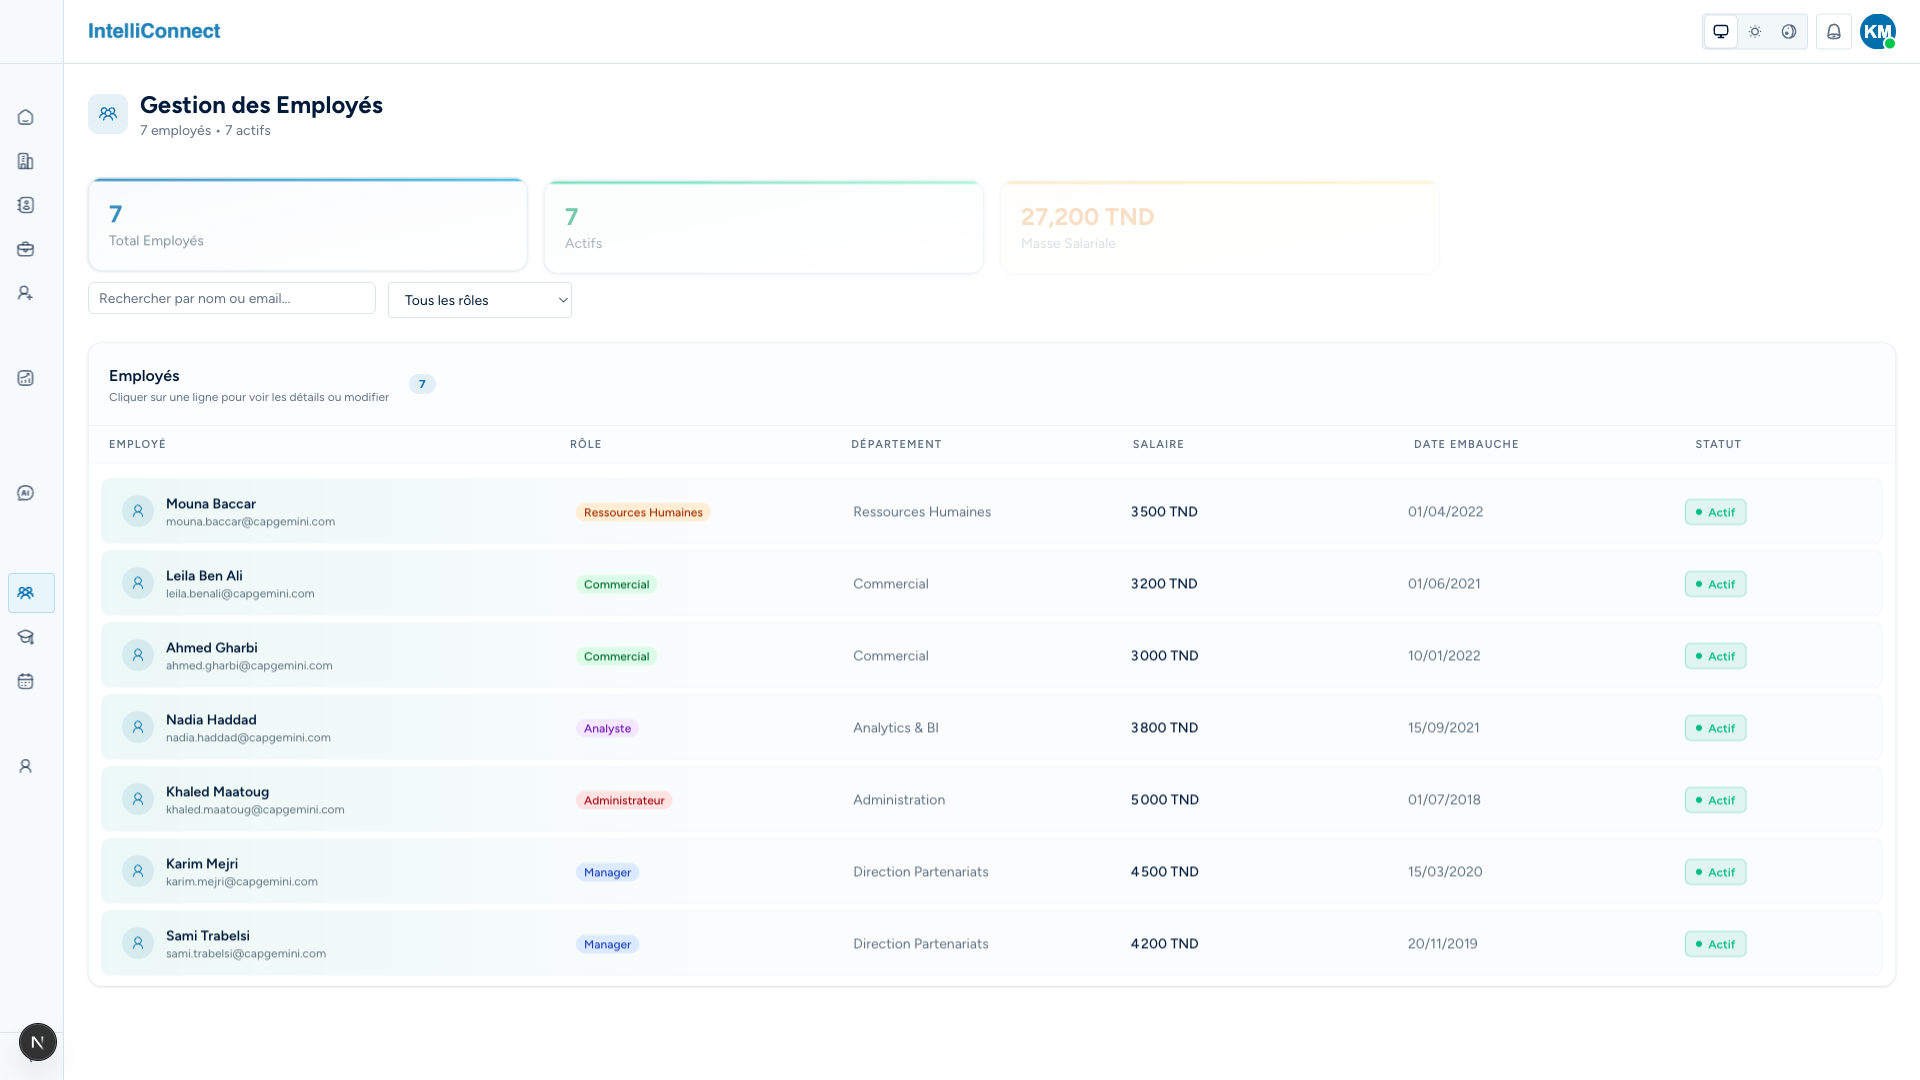
\includegraphics[width=\linewidth,height=0.18\textheight,keepaspectratio]{figures/screenshots/print/hr-employees-16x9.png}}\\[2pt]
    {\scriptsize Employee roster and role context}
  \end{minipage}\hfill
  \begin{minipage}[t]{0.48\linewidth}
    \centering
    \fbox{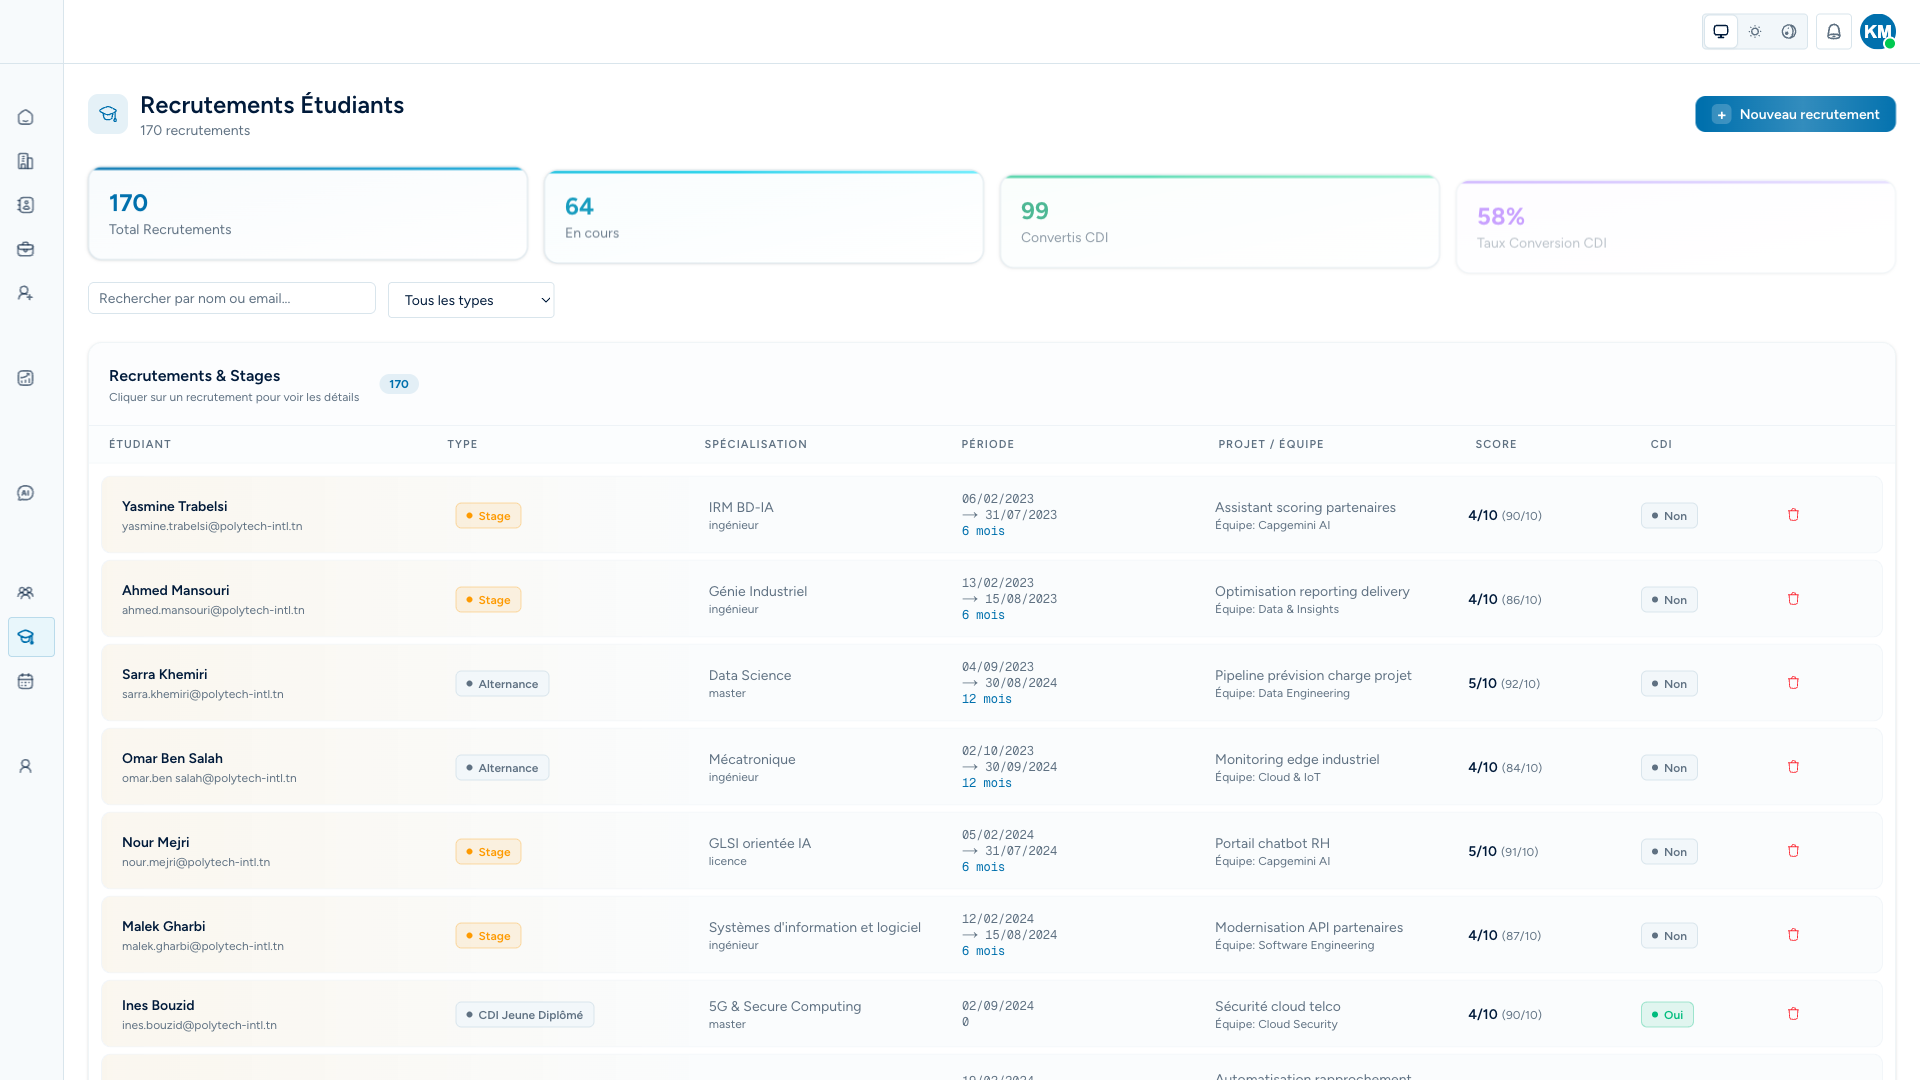
\includegraphics[width=\linewidth,height=0.18\textheight,keepaspectratio]{figures/screenshots/print/hr-recruitments-16x9.png}}\\[2pt]
    {\scriptsize Student recruitment and CDI conversions}
  \end{minipage}

  \vspace{0.5em}

  \begin{minipage}[t]{0.48\linewidth}
    \centering
    \fbox{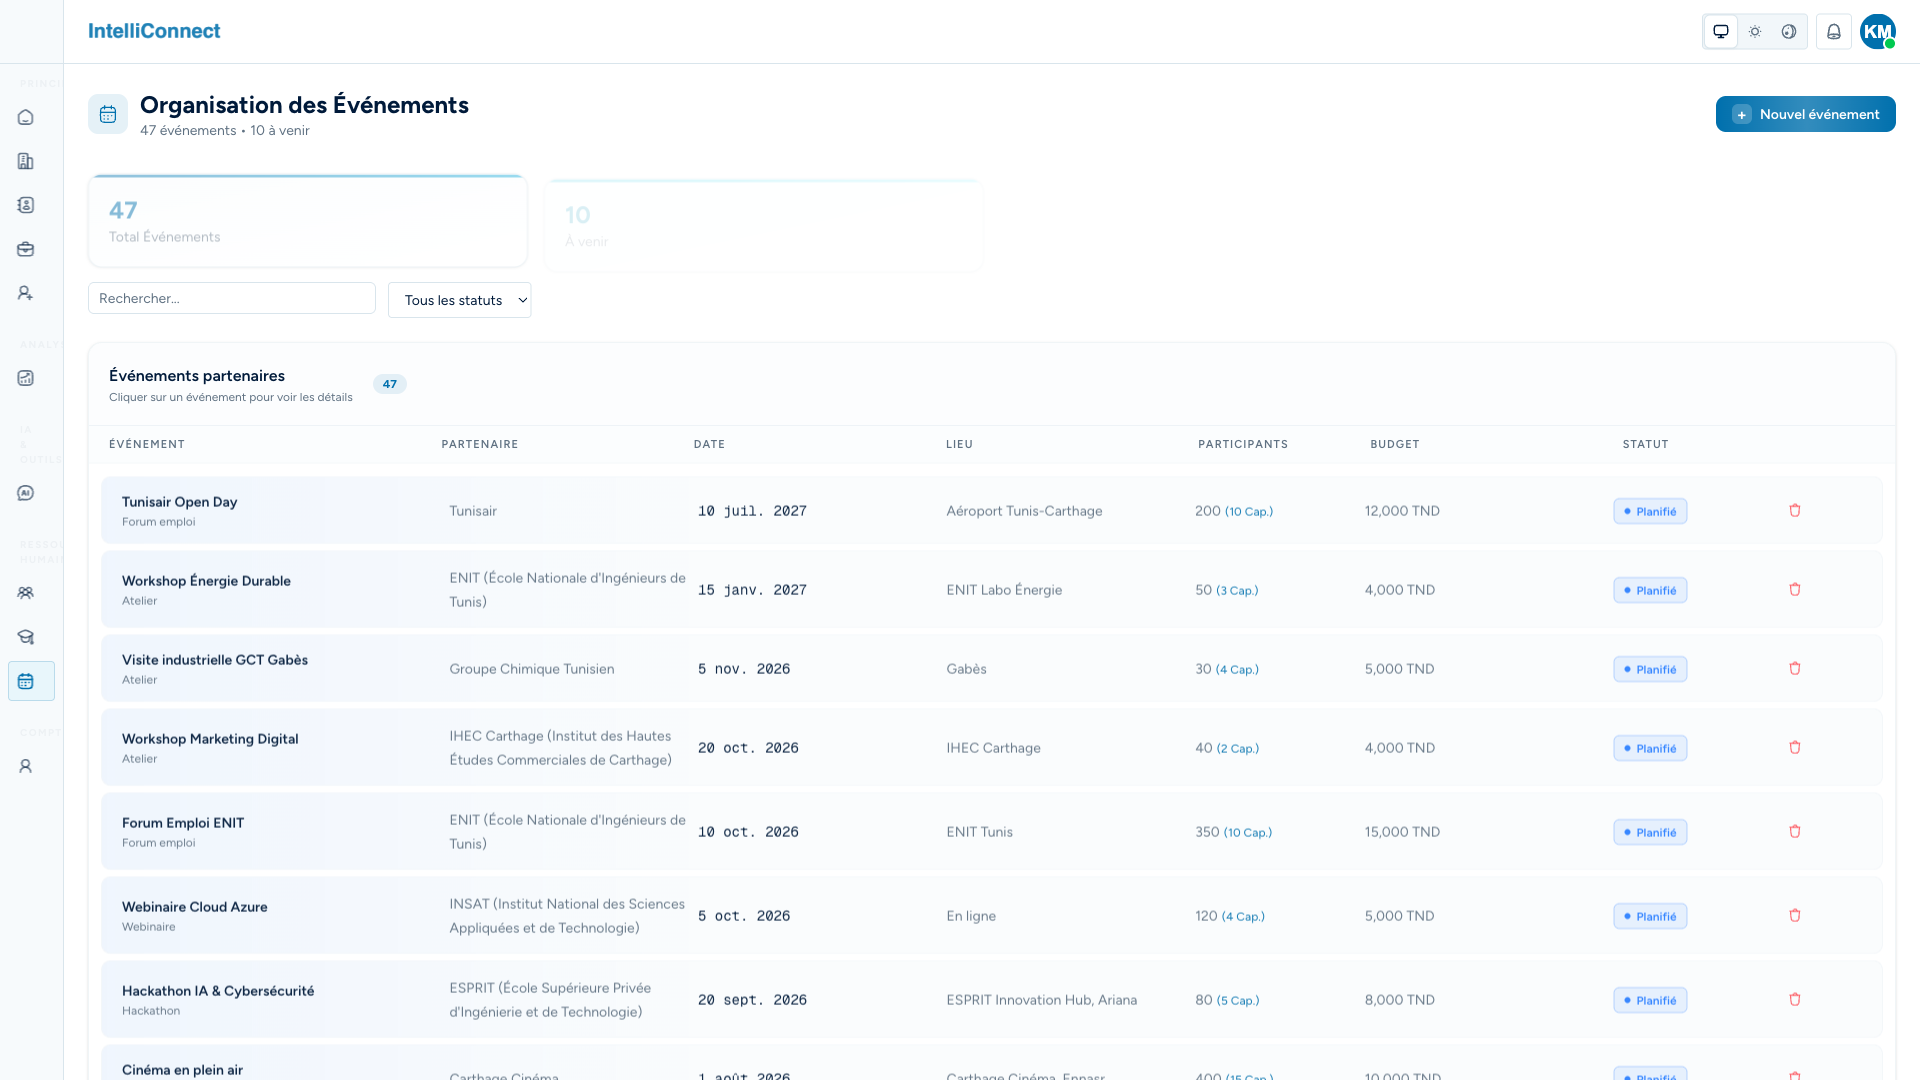
\includegraphics[width=\linewidth,height=0.18\textheight,keepaspectratio]{figures/screenshots/print/hr-events-16x9.png}}\\[2pt]
    {\scriptsize HR events organizer}
  \end{minipage}\hfill
  \begin{minipage}[t]{0.48\linewidth}
    \centering
    \fbox{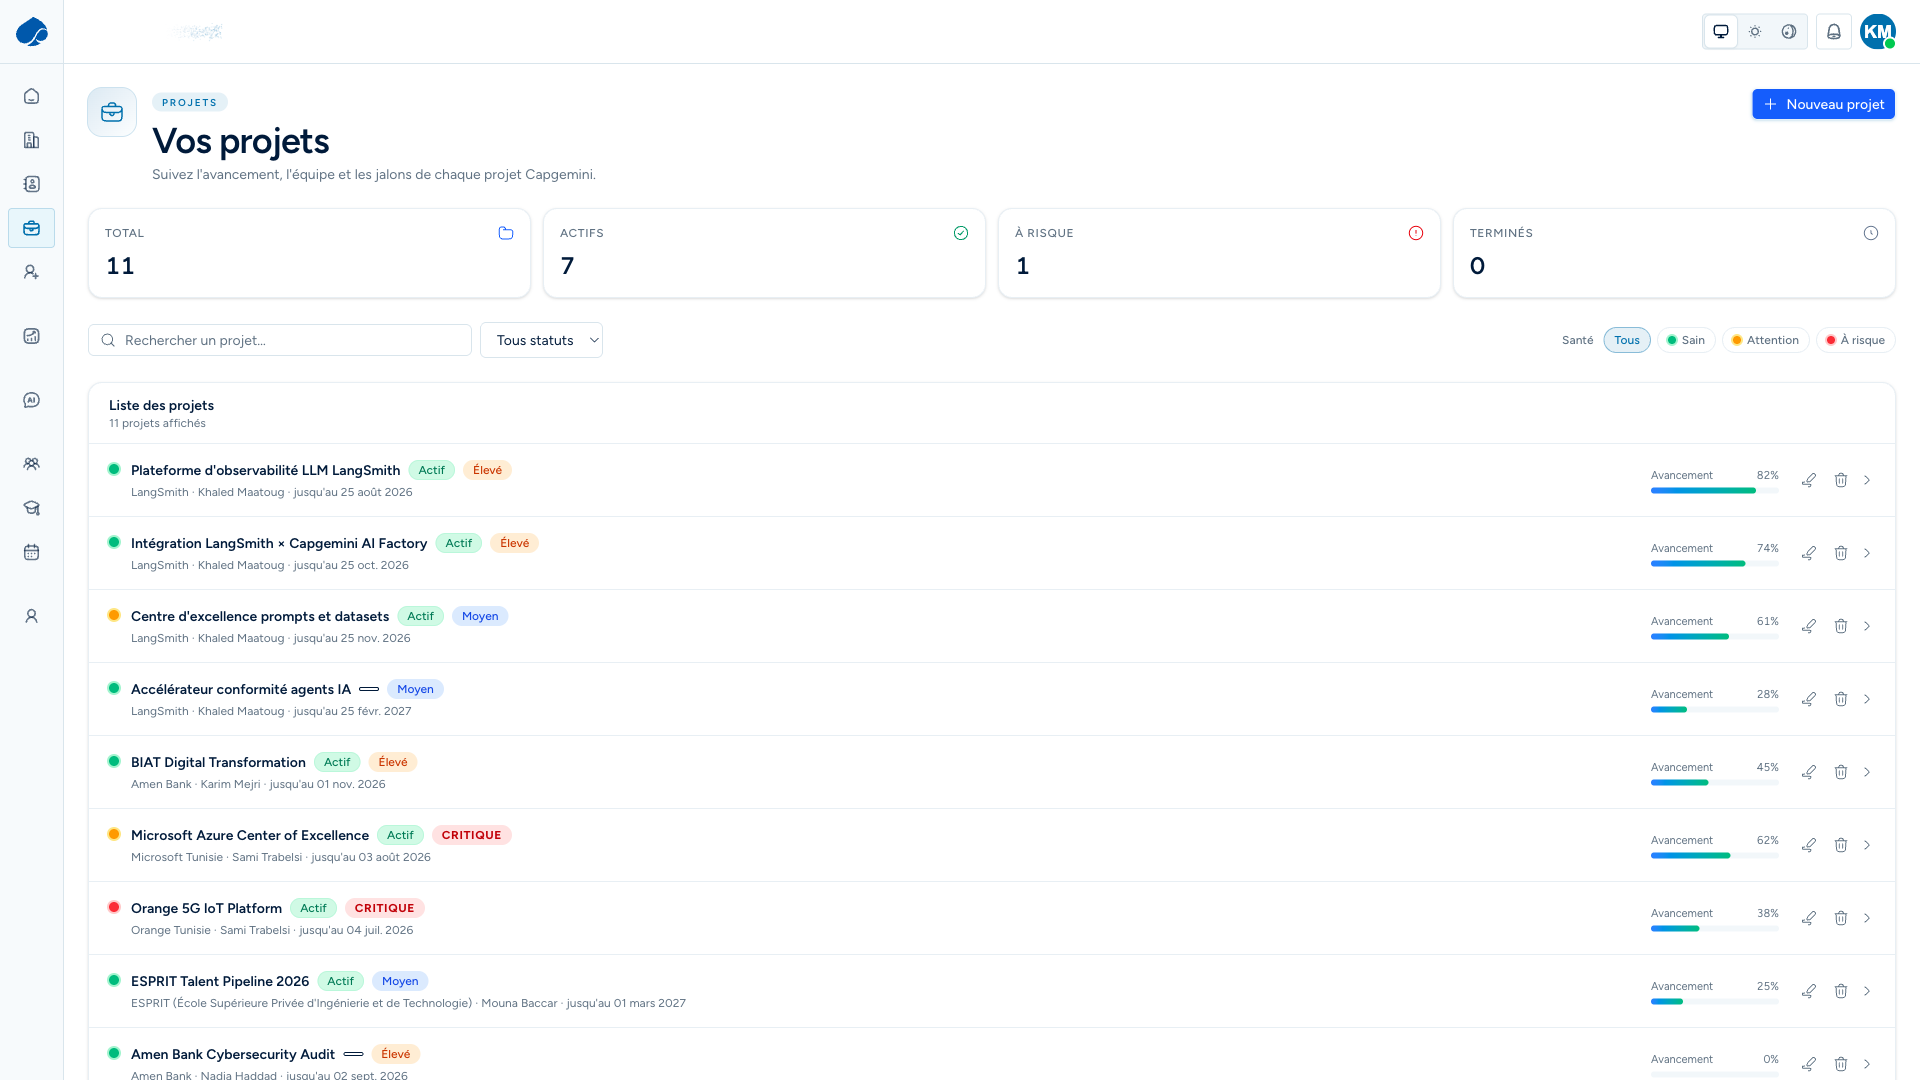
\includegraphics[width=\linewidth,height=0.18\textheight,keepaspectratio]{figures/screenshots/print/projects-list-16x9.png}}\\[2pt]
    {\scriptsize Project portfolio health and progress}
  \end{minipage}
  \caption{HR and delivery integration views. Employee records, recruitment outcomes, events, and project health are presented as connected operational signals rather than separate HR administration screens.}
  \label{fig:hr-delivery-views}
\end{figure}

\subsection{University Student Recruitment and CDI Conversion Signals}

The university-recruitment pipeline tracks students from initial contact through internship and permanent employment. Each record carries the student profile, specialization, associated partner institution, matching score, and outcome. For university partners such as ESPRIT and Polytech Intl, the pipeline measures partnership depth: how many students were converted to CDI is a direct indicator of the value the academic relationship delivers to Capgemini. These CDI conversion signals feed the partner scoring model through the \textit{track record} dimension, making the academic partnership pipeline a quantitative input to the broader scoring and ranking system.
For the report, this choice is important because university partnerships are not evaluated only by meetings or event counts. They also produce measurable talent outcomes. A school that regularly generates qualified internship candidates, converts students to permanent contracts, and stays active in events contributes directly to the long-term value of the partnership. The HR-readiness module therefore treats recruitment indicators as partnership signals, not as isolated HR administration.

The current implementation remains intentionally bounded. It exposes the indicators required for demonstration and scoring, while the deeper recruitment workflow is left to the dedicated HR/recruitment sister project. This keeps \projectname{} focused on partnership governance and avoids duplicating a complete HR product, but still leaves a clear integration path for future data exchange.
\subsection{Future Integration with Capgemini's HR/Recruitment Sister Project}
\begin{table}[H]
  \centering
  \caption{HR and recruitment integration roadmap}\label{tab:hr-roadmap}
  \begin{tabularx}{\textwidth}{>{\raggedright\arraybackslash}p{3.2cm}>{\raggedright\arraybackslash}p{4.4cm}X}
    \toprule
    Phase & Scope & Expected result \\
    \midrule
    Current foundation & Employee roster, employee statistics, internal events and project allocations. & \projectname{} can support delivery staffing and basic people-related dashboards without becoming a full HR system. \\
    Controlled data exchange & Import aggregated university student recruitment indicators and CDI conversion counts from the HR/recruitment sister project. & Academic partnership performance becomes measurable through trusted talent-outcome signals. \\
    Staffing intelligence & Use employee skills, availability and allocation load to recommend staffing options for partner projects. & Managers can identify suitable internal contributors with lower manual effort. \\
    Strategic BI alignment & Combine partner, project, budget, event, university student recruitment and CDI conversion facts in the data warehouse. & BI dashboards can correlate partnership activity with delivery and talent outcomes. \\
    Governance and audit & Define access rules, synchronization logs and data minimization policies for exchanged HR/recruitment data. & The integration remains secure, explainable and limited to business-relevant indicators. \\
    \bottomrule
  \end{tabularx}
\end{table}
\section{Conclusion}
This chapter presented the delivery and operations layer of \projectname{}. The project portfolio gives managers an overview of active initiatives, while the project detail page provides the evidence needed for execution: health, progress, budget, schedule, milestones, mini tasks, team allocations, and documents. The BI dashboard uses a separate data warehouse and server-side aggregation, reports complete the decision-support flow, and the HR module remains a light integration point with Capgemini's HR/recruitment sister project for university student recruitment and CDI conversion data.
